\chapter{XML Modeling Extension} \label{ch:xmlparser}

Modeling complex human-machine systems is a very difficult and time-consuming task.  This is evidenced by the shear number of modeling approaches to systems involving humans (ACT-R, Soar, DIARC, Brahms, EOFM), the panel ``Modeling Hurts'' at the upcoming AAAI workshop on Formal Methods in Human-Machine Systems, and our own experiences in generating the UE-WiSAR models.  By constructing the MAF Modeling Interface as a set of Java interfaces and abstract classes it meant that the framework was almost entirely extensible in any direction.  We found this very refreshing during the first few development iterations of the framework and model.  We quickly began creating Actors, sub-Actors, Events, States, and Transitions.  Eventually as our model grew in size and complexity the freedom of the Java language became a dual edged sword.  Our model was full of implicit declarations, inconsistencies, duplicated code, and anonymous methods; unbound functions with access to local scope which can be declared in-line which can make debugging more difficult.  It became extremely difficult to maintain the model let alone add to it.  More importantly, it became almost impossible to know if the models were valid and error-free.  This also made it difficult to rely on the metrics we were gathering as each Actor and Transition could implement metric reporting differently.  This chapter discusses an approach to creating MAF models which reduce these problems.

\section{Modeling Approach}

One approach for improving modeling efficiency is to create GUIs which help the user visualize the model in a way which allows them to more easily understand and make changes to the model.  An example of this is the Brahms Composer~\cite{seah2005multi} which allows the user to create models on the GUI and to visualize the model in different ways.  Another simpler approach is to use a language structure which is human readable and facilitates the creation of an accurate mental model.  An example of this is EOFM~\cite{bolton2009enhanced} which uses an XML structure which can be visualized as a tree graph.  The last approach we will mention is the use of design patterns and object oriented principles to build models which do not exhibit these problems.  The downside to this approach is it requires expert Java programming skills to build error-free models.

While others have successfully taken the third approach, for this thesis we chose to take an approach similar to that of EOFM by constructing an XML structure which represents a labeled state transition system.  Unlike EOFM the XML structure is not the main modeling language.  The XML structure represents a subset of the MAF language which is represented by the underlying Java objects which implement the MAF Modeling Interface.  We chose this approach for several reasons:  XML is commonly used for modeling and other similar tasks~\cite{bolton2009enhanced}, it is simple to work with in Java, it is human readable, and it is structured.  This gave us confidence that we would be able to represent any model in XML, perform validation on the model, and then convert the model into Java.  We also chose this approach because the XML is semantically constrained to the structure we define.  The modeler needs only a basic understanding of XML structures and the defined modeling semantics to implement a model.  Another reason for this approach was that it matches the MAF design.  MAF represents a top down approach to abstraction, meaning that the top level Actors, States, Transitions, and Channels are very abstract.  Each subsequent layer removes a portion of that abstraction.  The XML modeling extension adds constraints to the top level Modeling Interface which are designed to remove unwanted abstraction from the modeling language itself.  In this case that abstraction was in the form of unnecessary modeling capabilities.

\section{XML Structure}

We defined the following XML structure to represent the LSTS which is sent to the Simulator.  

The root node is the {\em \textless team\textgreater} element which consists of the {\em name} attribute and three child elements: {\em \textless channels\textgreater}, {\em \textless actors\textgreater}, and {\em \textless events\textgreater}.

\begin{spacing}{.5}
\lstinputlisting[language=XML]{xml_team.xml}
\end{spacing}

\subsection{Channels}

The {\em \textless channels\textgreater} element represents the DiTG and is comprised of any number of {\em \textless channel\textgreater} elements.  Each {\em \textless channel\textgreater} element represents a single uni-directional communication channel between a source Actor and a target Actor with attributes for the name, type, source, target, and optional dataType.  This is the only location in the XML that defines channels.  Every other {\em \textless channel\textgreater} element references one of these channels by using the channel name as its value.

\begin{spacing}{.5}
\lstinputlisting[language=XML]{xml_channels.xml}
\end{spacing}

\subsection{Actors}

The {\em \textless actors\textgreater} element represents the DiRGs contained in the model and is comprised of one or more {\em \textless actor\textgreater} elements.  Each {\em \textless actor\textgreater} has a {\em name} attribute, which must be unique, and a {\em showMetrics} attribute and is made up of several child elements.  The {\em \textless inputchannels\textgreater} and {\em \textless outputchannels\textgreater} elements are placed here to validate the DiTG.  The {\em actor} may have 0 or more {\em memory} elements which represent declarative memory used internally as part of the labeled state transitions.  The {\em \textless actor\textgreater} contains a list of 1 or more {\em \textless state\textgreater} elements inside of the {\em \textless states\textgreater} element.  Additionally the {\em \textless actor\textgreater} element must contain a single {\em \textless startState\textgreater} element with a value that matches the name attribute of one of the {\em \textless states\textgreater} child elements.

\begin{spacing}{.5}
\lstinputlisting[language=XML]{xml_actors.xml}
\end{spacing}


\subsection{States and Transitions}

The {\em \textless state\textgreater} element represents the `State' in the LSTS.  Each {\em \textless state\textgreater} element has a {\em name} attribute, which must be unique to the parent {\em \textless actor\textgreater} element, and a {\em load} attribute with a value of 0-4, we will discuss state load in the next chapter.  The {\em \textless state\textgreater} element also contains 0 or more {\em \textless transition\textgreater} child elements .  If no {\em \textless transition\textgreater} child elements are specified then it is an end state.  

The {\em \textless transition\textgreater} element represents the `Transition' in the LSTS and is composed of {\em durationMin} and {\em durationMax} attributes which are used for the transition duration range.  It also has a {\em priority} attribute which is used to rank a transitions priority with respect to the other state transitions.  Each {\em \textless transition\textgreater} element contains four child elements: {\em \textless description\textgreater}, {\em \textless inputs\textgreater}, {\em \textless outputs\textgreater}, and {\em \textless endState\textgreater}.  

The {\em \textless description\textgreater} element value contains a description of the transition which is meant to help give the modeler insight into what the transition is actually doing.  It is also used in the debug logs to help track down modeling errors.  

The {\em \textless inputs\textgreater} and {\em \textless outputs\textgreater} elements represent the `Label' in the LSTS.  These elements contain 0 or more {\em \textless memory\textgreater} and {\em \textless channel\textgreater} elements.  All {\em \textless inputs\textgreater} element children have a {\em name} attribute, a {\em predicate} attribute, an optional {\em dataType} attribute and a value.  If the child element is a {\em \textless channel\textgreater} then it may optionally declare only the {\em name} attribute and 1 or more {\em \textless layer\textgreater} child elements which declare {\em name}, {\em predicate}, and optional {\em dataType} attributes along with a value.  The {\em \textless channel\textgreater} name must correlate with an {\em \textless actor\textgreater} {\em \textless inputchannels\textgreater} {\em \textless channel\textgreater} value.  The {\em predicate} attribute contains one of six predicate values: equal to, not equal, greater than, less than, greater than or equal, or less than or equal.  The {\em dataType} is one of three options: String, Integer, or Boolean with a default of String.  The value of these child elements is the value which will be compared against the channel or memory value.  

The {\em \textless outputs\textgreater} element is similar to the {\em \textless inputs\textgreater} element except that its children do not specify {\em predicate} or {\em dataType} attributes.  

This structure allows the modeler to use a 2 dimensional labeling system.  The first dimension being the direction of the data flow, input or output.  The second dimension being the source of the data; channel, layer, or memory.  This allows the LSTS to be very flexible while using a relatively simple syntax.  We should also point out that the transition {\em \textless inputs\textgreater} element contains the following propositional logic: $(Child_{1} \bigwedge Child_{2} \bigwedge \ldots \bigwedge Child_{n})$ which forces the modeler to create a new {\em \textless transition\textgreater} element for each label.

The value of the{\em \textless endState\textgreater} element contains the name of the Actors ending state if this transition were applied.  This value cannot be empty and must match an existing {\em \textless state> name}.

\begin{spacing}{.5}
\lstinputlisting[language=XML]{xml_state_transition.xml}
\end{spacing}


\subsection{Events}

The {\em \textless events\textgreater} element contains a child {\em \textless event\textgreater} element for each unique type of event the system can experience.  The {\em \textless event\textgreater} has a {\em name} attribute, must be unique, and a {\em count} attribute which determines how many times the Simulator will fire the event.  Each {\em \textless event\textgreater} element defines a single {\em \textless transition\textgreater} element which differs from the previously mentioned transition element in that it does not define duration, priority, or an end state.

\begin{spacing}{.5}
\lstinputlisting[language=XML]{xml_events.xml}
\end{spacing}

\section{XML Model Parser}

With the XML structure defined we then moved onto parsing the XML.  See figure~\ref{fig:xml_model_extension}.  To accomplish this we created a Java class named XMLModelParser.  This class performed two main functions.  The first was to create the necessary Java objects and the second was to perform basic error checking on the model.  

The XMLModelParser works by first loading the XML model into an XML object.  This allows us to search the XML structure for specific elements and attributes.  The structure of the XML model facilitates the parsing effort since each child element is also a child object.  The first object which is created is the Team.  Next the DiTG is added to the team by creating ComChannel objects for each channel.  The Actor parsing is the most complex.  Each actor element defines its own DiTG, memory, states, transitions, and labels.  One of the challenges with the Actor parsing was ensuring that the Java objects were constructed in an order which allowed them to link properly.

\begin{figure}[h]
\begin{center}
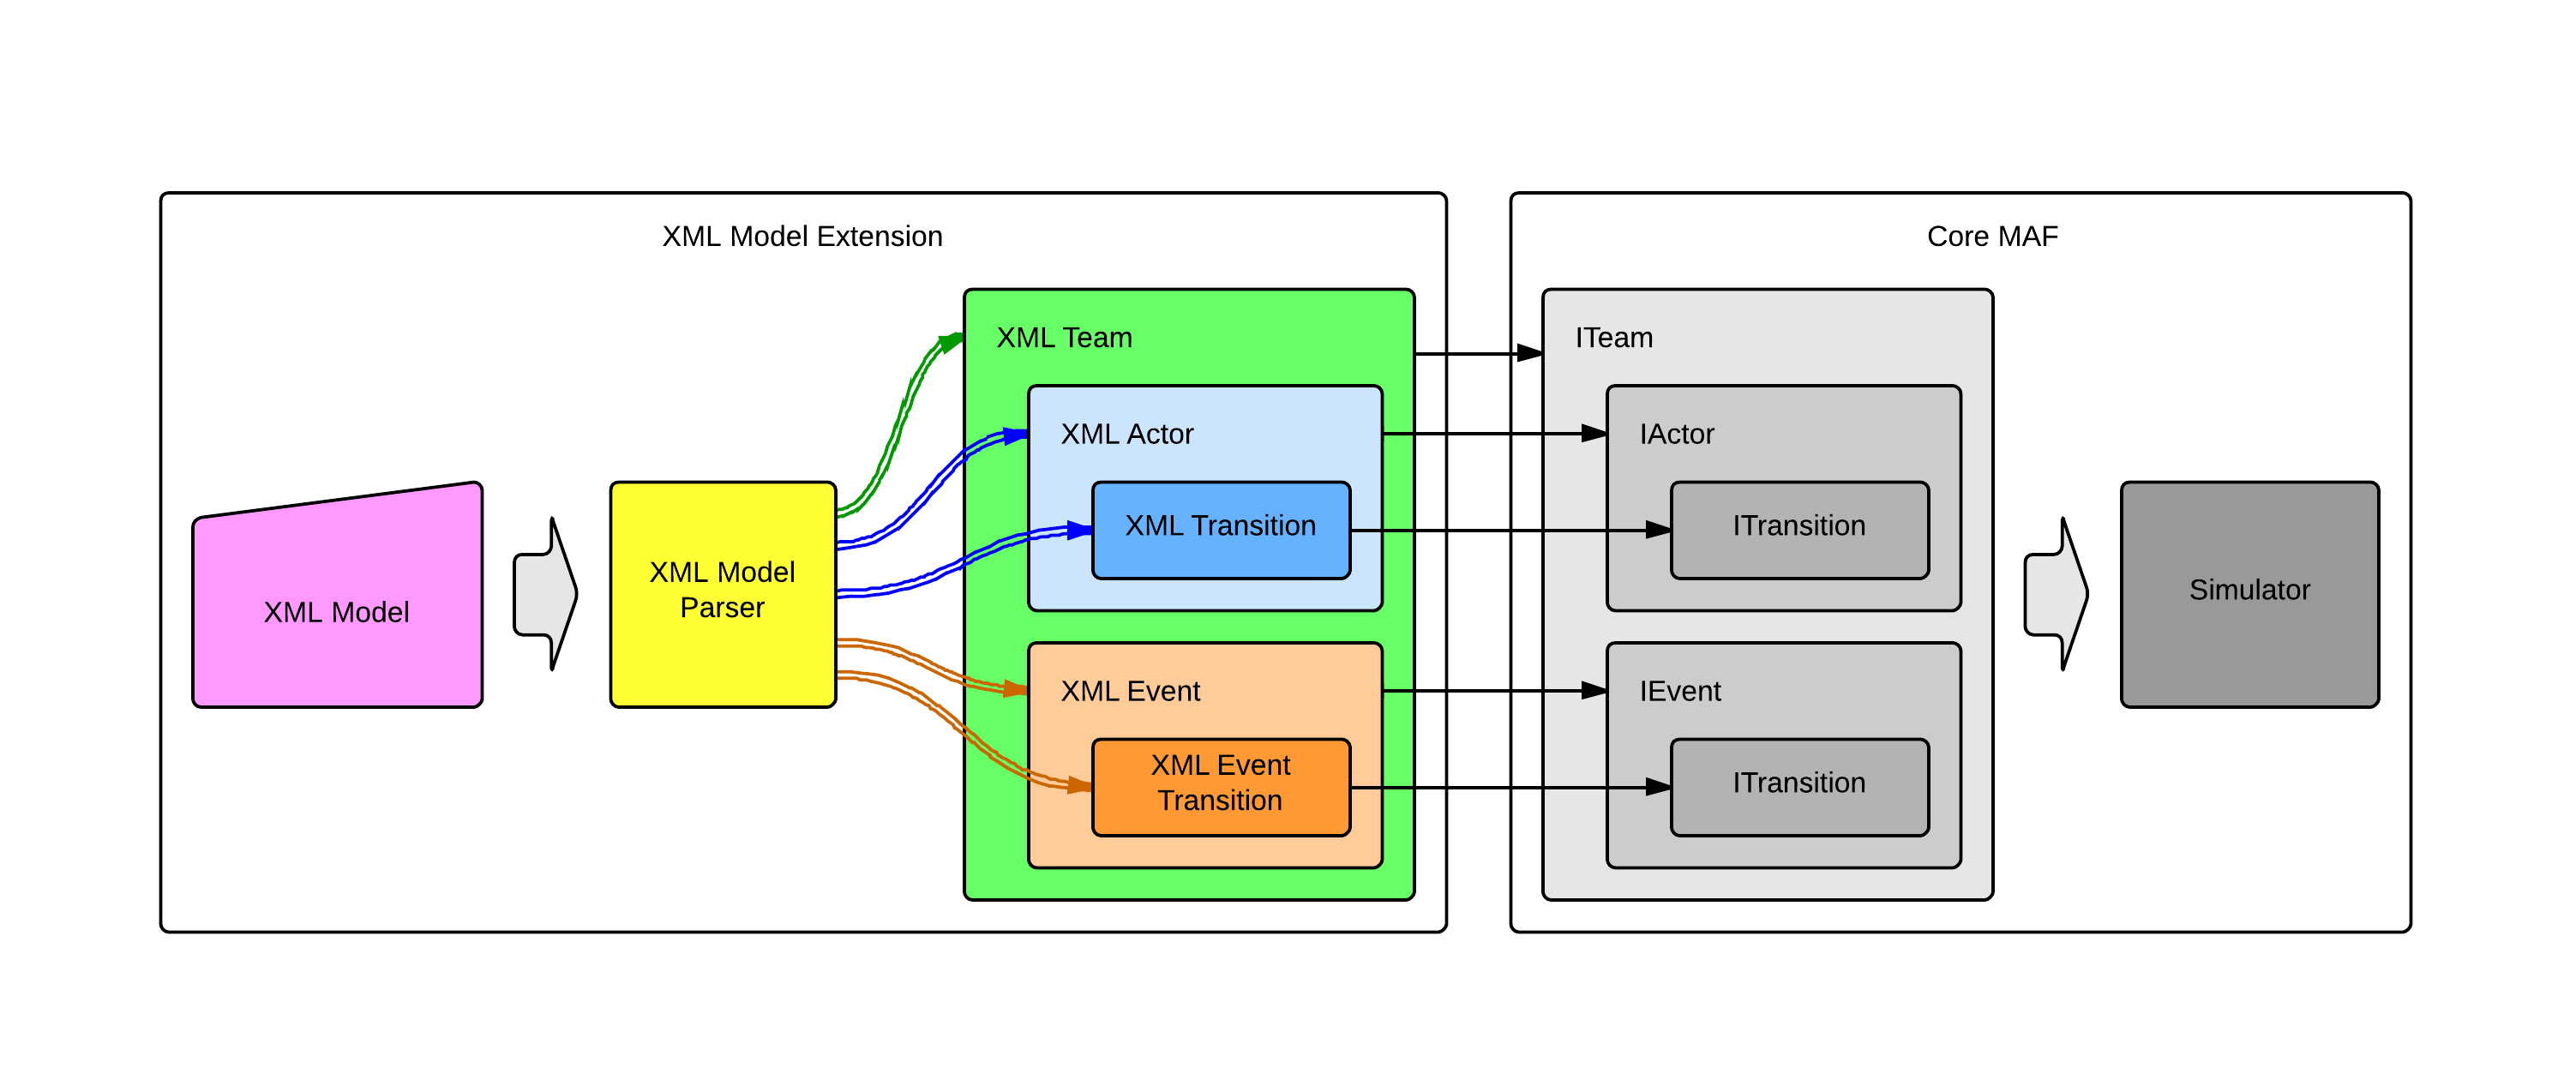
\includegraphics[width=6in]{xml_model_extension.png}
\caption{XML Model Extension Breakdown}
\label{fig:xml_model_extension}
\end{center}
\end{figure}

\subsection{Attaching to the Simulator}

To pass a valid LSTS to the Simulator the XMLModelParser must construct Java classes which implement the MAF Modeling Interface.  To accomplish this we created a set of generic XML classes, each class implements a specific portion of the Modeling Interface such as the ITransition or IActor interfaces.  These interfaces allow the Simulator to query and execute transitions on the LSTS.  The list of XML classes includes the XMLTeam, XMLActor, XMLTransition, XMLEvent, XMLEventTransition and other helper classes.  A link to the source code can be found in appendix~\ref{code}.  Each of these generic XML classes lies separate from the core simulation code.  This means that the addition of the XML parser does not prevent the use of custom Actors or Transition classes, use of a different model parser, or extension of our existing XML parser.  In fact our XML model extension is meant to be expanded to handle a more robust set of models.   As we developed a model using this XMLModelParser we had several occasions to extend its capabilities which we discuss later.  Unsurprisingly it was not difficult to extend the XML to accommodate the changes, often requiring less than 100 lines of code (not including changes to the model XML).

\subsection{Validation}

One of the most time consuming aspects of the modeling process was validating that the model was correct.  By correct we mean that each designed path through the model can and will be traversed when given a specific set of inputs.  In order to ensure that the model was correct we had to manually step through the model simulation paths during construction and check that the correct paths were being taken.  According to commit dates in our github repository we estimate that our initial 5 Actor sample model took three days to create and validate.  The following 12 Actor fully functional model took 34 days to create and validate.  However, the fully functional model only contained $4\times$ the amount of code.  See figure~\ref{fig:time_to_model}~\footnote{In figure~\ref{fig:time_to_model} time to model is an approximation generated by analyzing github commits.  Also lines of code has been adjusted to account for whitespace, comments, and lines with fewer than 5 characters.}.  The discrepancy between the time to model and the model size demonstrates how problematic model validation can become as model complexity increases.

\begin{figure}[h]
\begin{center}
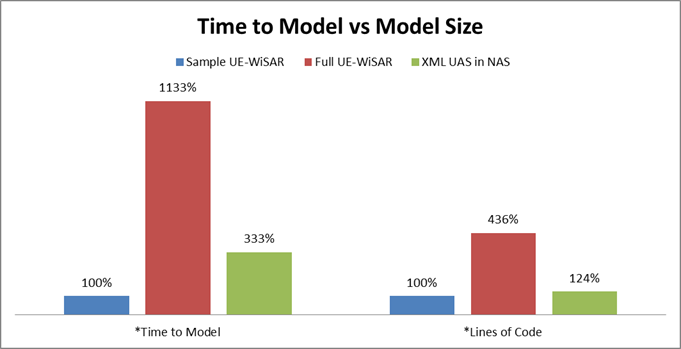
\includegraphics[width=5in]{time_to_model.png}
\caption{Time to Model vs Model Size}
\label{fig:time_to_model}
\end{center}
\end{figure}

We observed several underlying modeling problems which we believe are responsible for the dramatic increase in validation time.  The first problem occurred when the modeler became disoriented while working within the model.  Each time a path branches or the modeler switches branches it becomes more likely that their mental model will diverge from the Java model.  As complexity increases the number of branches and the need to jump between branches also increases.  When this happens mistakes related to a divergent mental model, such as transitioning to the wrong state, forgetting to add a transition, or checking the wrong inputs, begin to appear.  Another problem was a lack of validation tools.  The step-through validation approach essentially meant that only a single modeling error could be found at a time and we had to step through the entire model for each error.  We also observed that modelers are prone to introduce common typing errors into the model which do not get caught by the Java compiler.  

The XML Modeling Extension helps to mitigate these problems in a few different ways.  The XML modeling structure is meant to help offset some of the complexity by presenting the model to the user in a more compact and semantically relevant form.  Java syntax such as class, new, void, etc\ldots are not relevant to the model and do not help the modeler understand the model.  The XML specific syntax however uses a much smaller footprint, additionally the structure itself describes the model in a very concise form which helps the modeler maintain a more accurate mental model which leads to fewer modeling errors.

This extension also helps by introducing a new validation tool.  The need to parse the XML into Java provides a natural location to perform basic error checking on the XML before creating the Java objects which are passed to the Simulator. The simple syntax and structure of the XML makes it much easier to check for user errors in the model.  One of the most common errors we found when creating the UAS integrated into NAS model was missing parameters.  Inside the XMLModelParser if a required portion of XML was not found an error was returned with a description of the problem and where it occurred.  The same was true for an invalid DiTG, duplicate element names, typos, and missing or impossible transitions.  This provided huge time savings when compared with the other alternatives of analyzing output logs or stepping through code with the debugger.

Another benefit introduced with this extension was the generic Java classes.  Each XML component had a single Java implementation.  This guaranteed that similar components would share the same behavior, something which Java interfaces do not provide.  It also meant that bugs in the Java code only needed to be fixed in a single location.

\section{Channel Layers}

While working on this extension it became apparent that our channel design was flawed.  From Threaded Cognition Theory~\cite{salvucci2008threaded} we are aware that an individual can perform multiple concurrent tasks that do not require an executive process.  It does not matter if those concurrent tasks originate from multiple sources or a single source, such as a GUI.  Our previous design restricted channels to a single type of data with no restriction as to what that data type was.  While an arbitrary data type allowed us to pass any amount of data, it made it very difficult to know what was really happening on the communication channel.  What we mean by this is that instead of explicitly defining concurrent tasks we rely on inputs and Actor state to imply that concurrent tasks are being performed.  The arbitrary data type thus prevented a single communication channel from implying multiple concurrent tasks.

To fix this flaw we decided to add layers to our communication channels. See figure~\ref{fig:layers}.  Each channel can have any number of layers.  For example, a visual channel from one person to another has two channels, one which analyzes the face and another which analyzes the body.  Their may be more accurate channel layering for this scenario but these layers satisfy this example.  When communication occurs on this visual channel the recipient can examine as many layers as are needed for the given state.  If the person is in a distracted state then maybe they are not looking at the face layer which may in turn reduce the probability of comprehending the corresponding audio channel.   Another good example where this is useful is in GUIs.  Each item that a GUI represents to the user can be represented as a different layer.  The more layers a GUI presents to a user the more complex it becomes which potentially makes it more difficult for a person to analyze, due to conflicting resources ~\cite{salvucci2008threaded}.

\begin{figure}[h]
\begin{center}
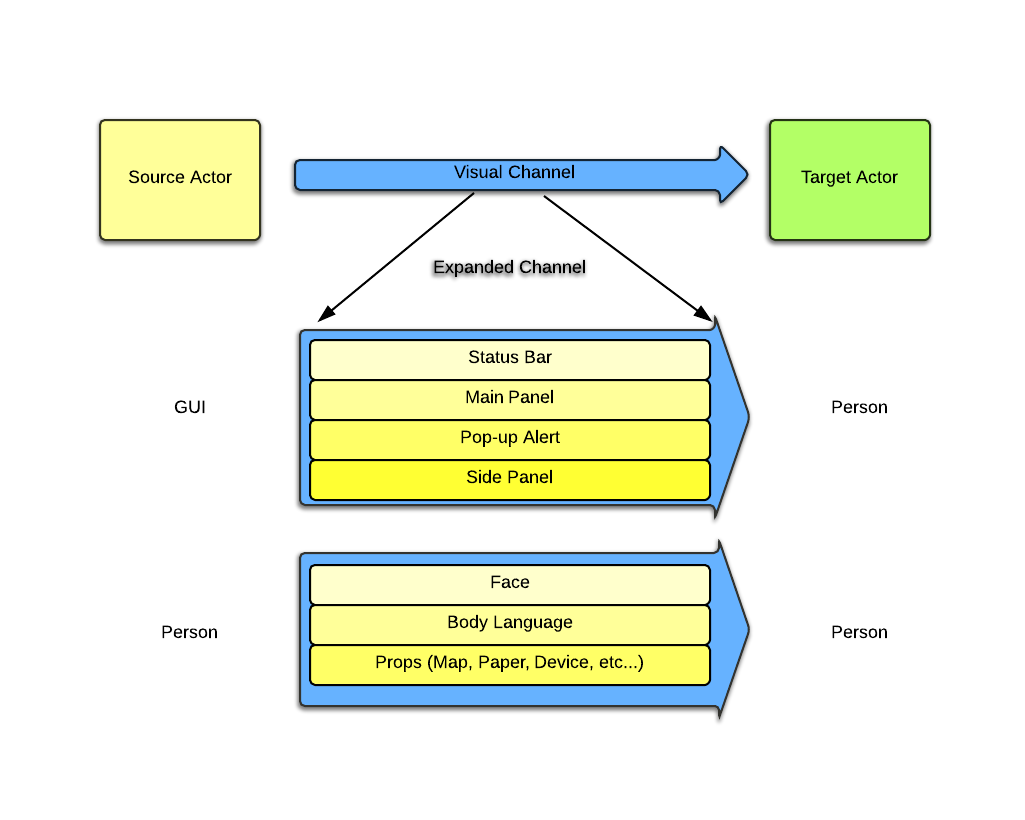
\includegraphics[width=5in]{layers.png}
\caption{Communication Channel Layers}
\label{fig:layers}
\end{center}
\end{figure}

We believe that this concept of channel layers creates a more natural flow of information across the DiTG while aligning MAF with modern human workload theory.  We also have the ability to perform a number of different measurements on the channel layers which, when combined with our other metrics, may prove valuable in obtaining accurate human workload measurements.

